% INVERSE HEAT CONDUCTION
Finally, an inverse heat conduction problem (IHCP) is considered.
The heat equation is a partial differential equation (PDE) that describes the distribution and evolution of heat in a system where conduction is the dominant mode of heat transfer.
We consider a stationary heat equation of the form
\begin{equation} \label{eq:JCP:Heat:Stationary}
  \nabla \cdot (\kappa \nabla \perfect{T}) = 0.
\end{equation}
The temperature is denoted as \(\perfect{T}\) and the thermal conductivity is denoted as \(\kappa\).
Commonly one is interested in the solution of the boundary value problem that is posed when \cref{eq:JCP:Heat:Stationary} is satisfied over a physical domain subject to appropriate boundary conditions.
We consider the steady state situation in two spatial dimensions.
The Euclidean coordinate vector is denoted as \(\bm{r} = (r_1,r_2)^\top\) in the following.
\par % PROBLEM SETUP
It is dealt with the identification of thermal conductivities of inclusions in a composite material with close-to-surface measurements of the temperature.
The setup of the simplified thermal problem is visualized in \cref{fig:JCP:Heat:HeatConduction2D}.
The thermal conductivity of the background matrix is denoted as \(\kappa_0\), while the conductivities of the material inclusions are termed as \(\kappa_1\) and \(\kappa_2\), respectively.
It is assumed that the material properties are not subject to a further spatial variability.
% BOUNDARY CONDITIONS
At the ``top'' of the domain a Dirichlet boundary condition \(\perfect{T}_1\) is imposed,
while at the ``bottom'' the Neumann boundary condition \(q_2 = - \kappa_0 \, \partial \perfect{T} / \partial r_2\) is imposed.
Zero heat flux conditions \(\partial \perfect{T} / \partial r_1 = 0\) are imposed at the ``left'' and ``right'' hand side.
\par % INVERSE PROBLEM
We consider the IHCP that is posed when the thermal conductivities \(\bm{\kappa} = (\kappa_1,\kappa_2)^\top\) are unknown and their inference is intended.
With this in mind, a number of \(\dimData\) measurements \(\bm{T} = (T(\bm{r}_1),\ldots,T(\bm{r}_\dimData))^\top\)
of the temperature field at the measurement locations \((\bm{r}_1,\ldots,\bm{r}_\dimData)\) is available.
The forward model \(\mathcal{M} \colon \bm{\kappa} \mapsto \perfect{\bm{T}}\) establishes the connection between the data and the unknowns.
It formalizes the operation of solving \cref{eq:JCP:Heat:Stationary} for \(\perfect{\bm{T}}\) as a function of \(\bm{\kappa}\).
Measured temperatures \(\bm{T} = \perfect{\bm{T}} + \bm{\varepsilon}\) consist of the corresponding model response \(\perfect{\bm{T}} = \mathcal{M}(\bm{\kappa})\) and a residual term \(\bm{\varepsilon}\).
The latter accounts for measurement uncertainty and forward model inadequacy.
We consider residuals that are distributed according to a Gaussian \(\mathcal{N}(\bm{\varepsilon} \cond \bm{0},\bm{\Sigma})\) with covariance matrix \(\bm{\Sigma}\).
In compliance with \cref{eq:JCP:Bayesian:Inverse:Likelihood} the likelihood function is given as \(\mathcal{L}(\bm{\kappa}) = \mathcal{N}(\bm{T} \cond \mathcal{M}(\bm{\kappa}),\bm{\Sigma})\).
Provided that a prior distribution \(\pi(\bm{\kappa})\) can be elicited, the posterior is given as \(\pi(\bm{\kappa} \cond \bm{T}) = \scale^{-1} \mathcal{L}(\bm{\kappa}) \pi(\bm{\kappa})\).
\par % EXPERIMENTAL SETUP
The thermal conductivity of the background matrix is set to \(\kappa_0 = \unit[15]{W/m/K}\),
while the thermal conductivities of the inclusions are specified as \(\kappa_1 = \unit[32]{W/m/K}\) and \(\kappa_1 = \unit[28]{W/m/K}\).
The material properties of the inclusions are treated as unknowns subsequently.
Moreover, the boundary conditions \(\perfect{T}_1 = \unit[200]{K}\) and \(q_2 = \unit[2000]{W/m^2}\) are imposed.
A finite element (FE) model is used to solve a weak form of the governing PDE.
The FE solution for the experimental setup described above is shown in \cref{fig:JCP:Heat:SteadyState2D}.
We consider a uniform prior distribution \(\pi(\bm{\kappa}) = \pi(\kappa_1) \pi(\kappa_2)\) with independent marginals
\(\pi(\kappa_1) = \mathcal{U}(\kappa_1 \cond \underline{\kappa}_1,\overline{\kappa}_1)\) and \(\pi(\kappa_2) = \mathcal{U}(\kappa_2 \cond \underline{\kappa}_2,\overline{\kappa}_2)\).
The prior bounds are chosen as \(\underline{\kappa}_1 = \underline{\kappa}_2 = \unit[20]{W/m/K}\) and \(\overline{\kappa}_1 = \overline{\kappa}_2 = \unit[40]{W/m/K}\), respectively.
A number of \(\dimData = 12\) close-to-surface observations is analyzed.
Their measurement locations are indicated by the black dots in \cref{fig:JCP:Heat:HeatConduction2D}.
Independent Gaussian measurement noise with \(\bm{\Sigma} = \sigma_T^2 \bm{1}\) and \(\sigma_T = \unit[0.25]{K}\) is considered.
Based on this setup, synthetic data are simulated for conducting the computer experiment.
This means that the forward model responses \(\perfect{\bm{T}}\) for the true parameter setup are computed and pseudo-random noise is added in order to obtain \(\bm{T}\).
% FIGURES: PDE & FEM
\begin{figure}[htbp]
  \begin{minipage}[b]{\JCPsubWidth}
    \centering
    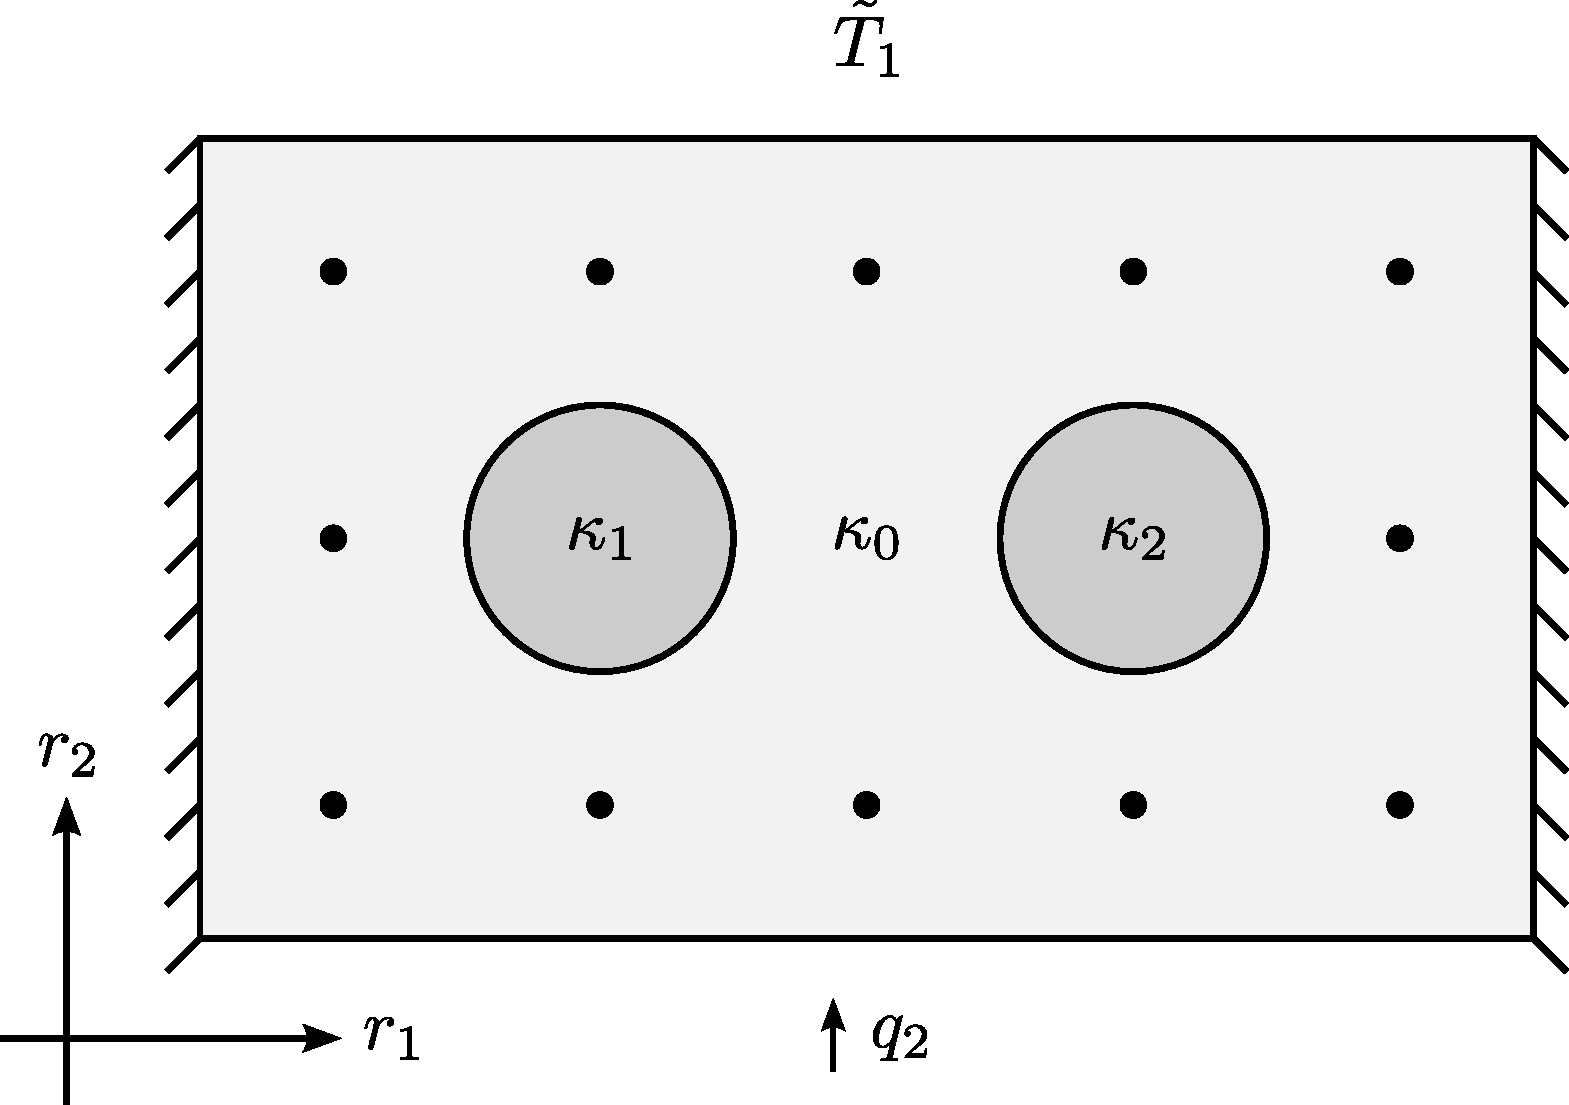
\includegraphics[height=\JCPfigHeight]{fig_JCP_Heat2D_HeatConduction}
    \caption[2D IHCP: Heat conduction setup]{2D IHCP: Heat conduction setup.}
    \label{fig:JCP:Heat:HeatConduction2D}
  \end{minipage}%
  \hfill%
  \begin{minipage}[b]{\JCPsubWidth}
    \centering
    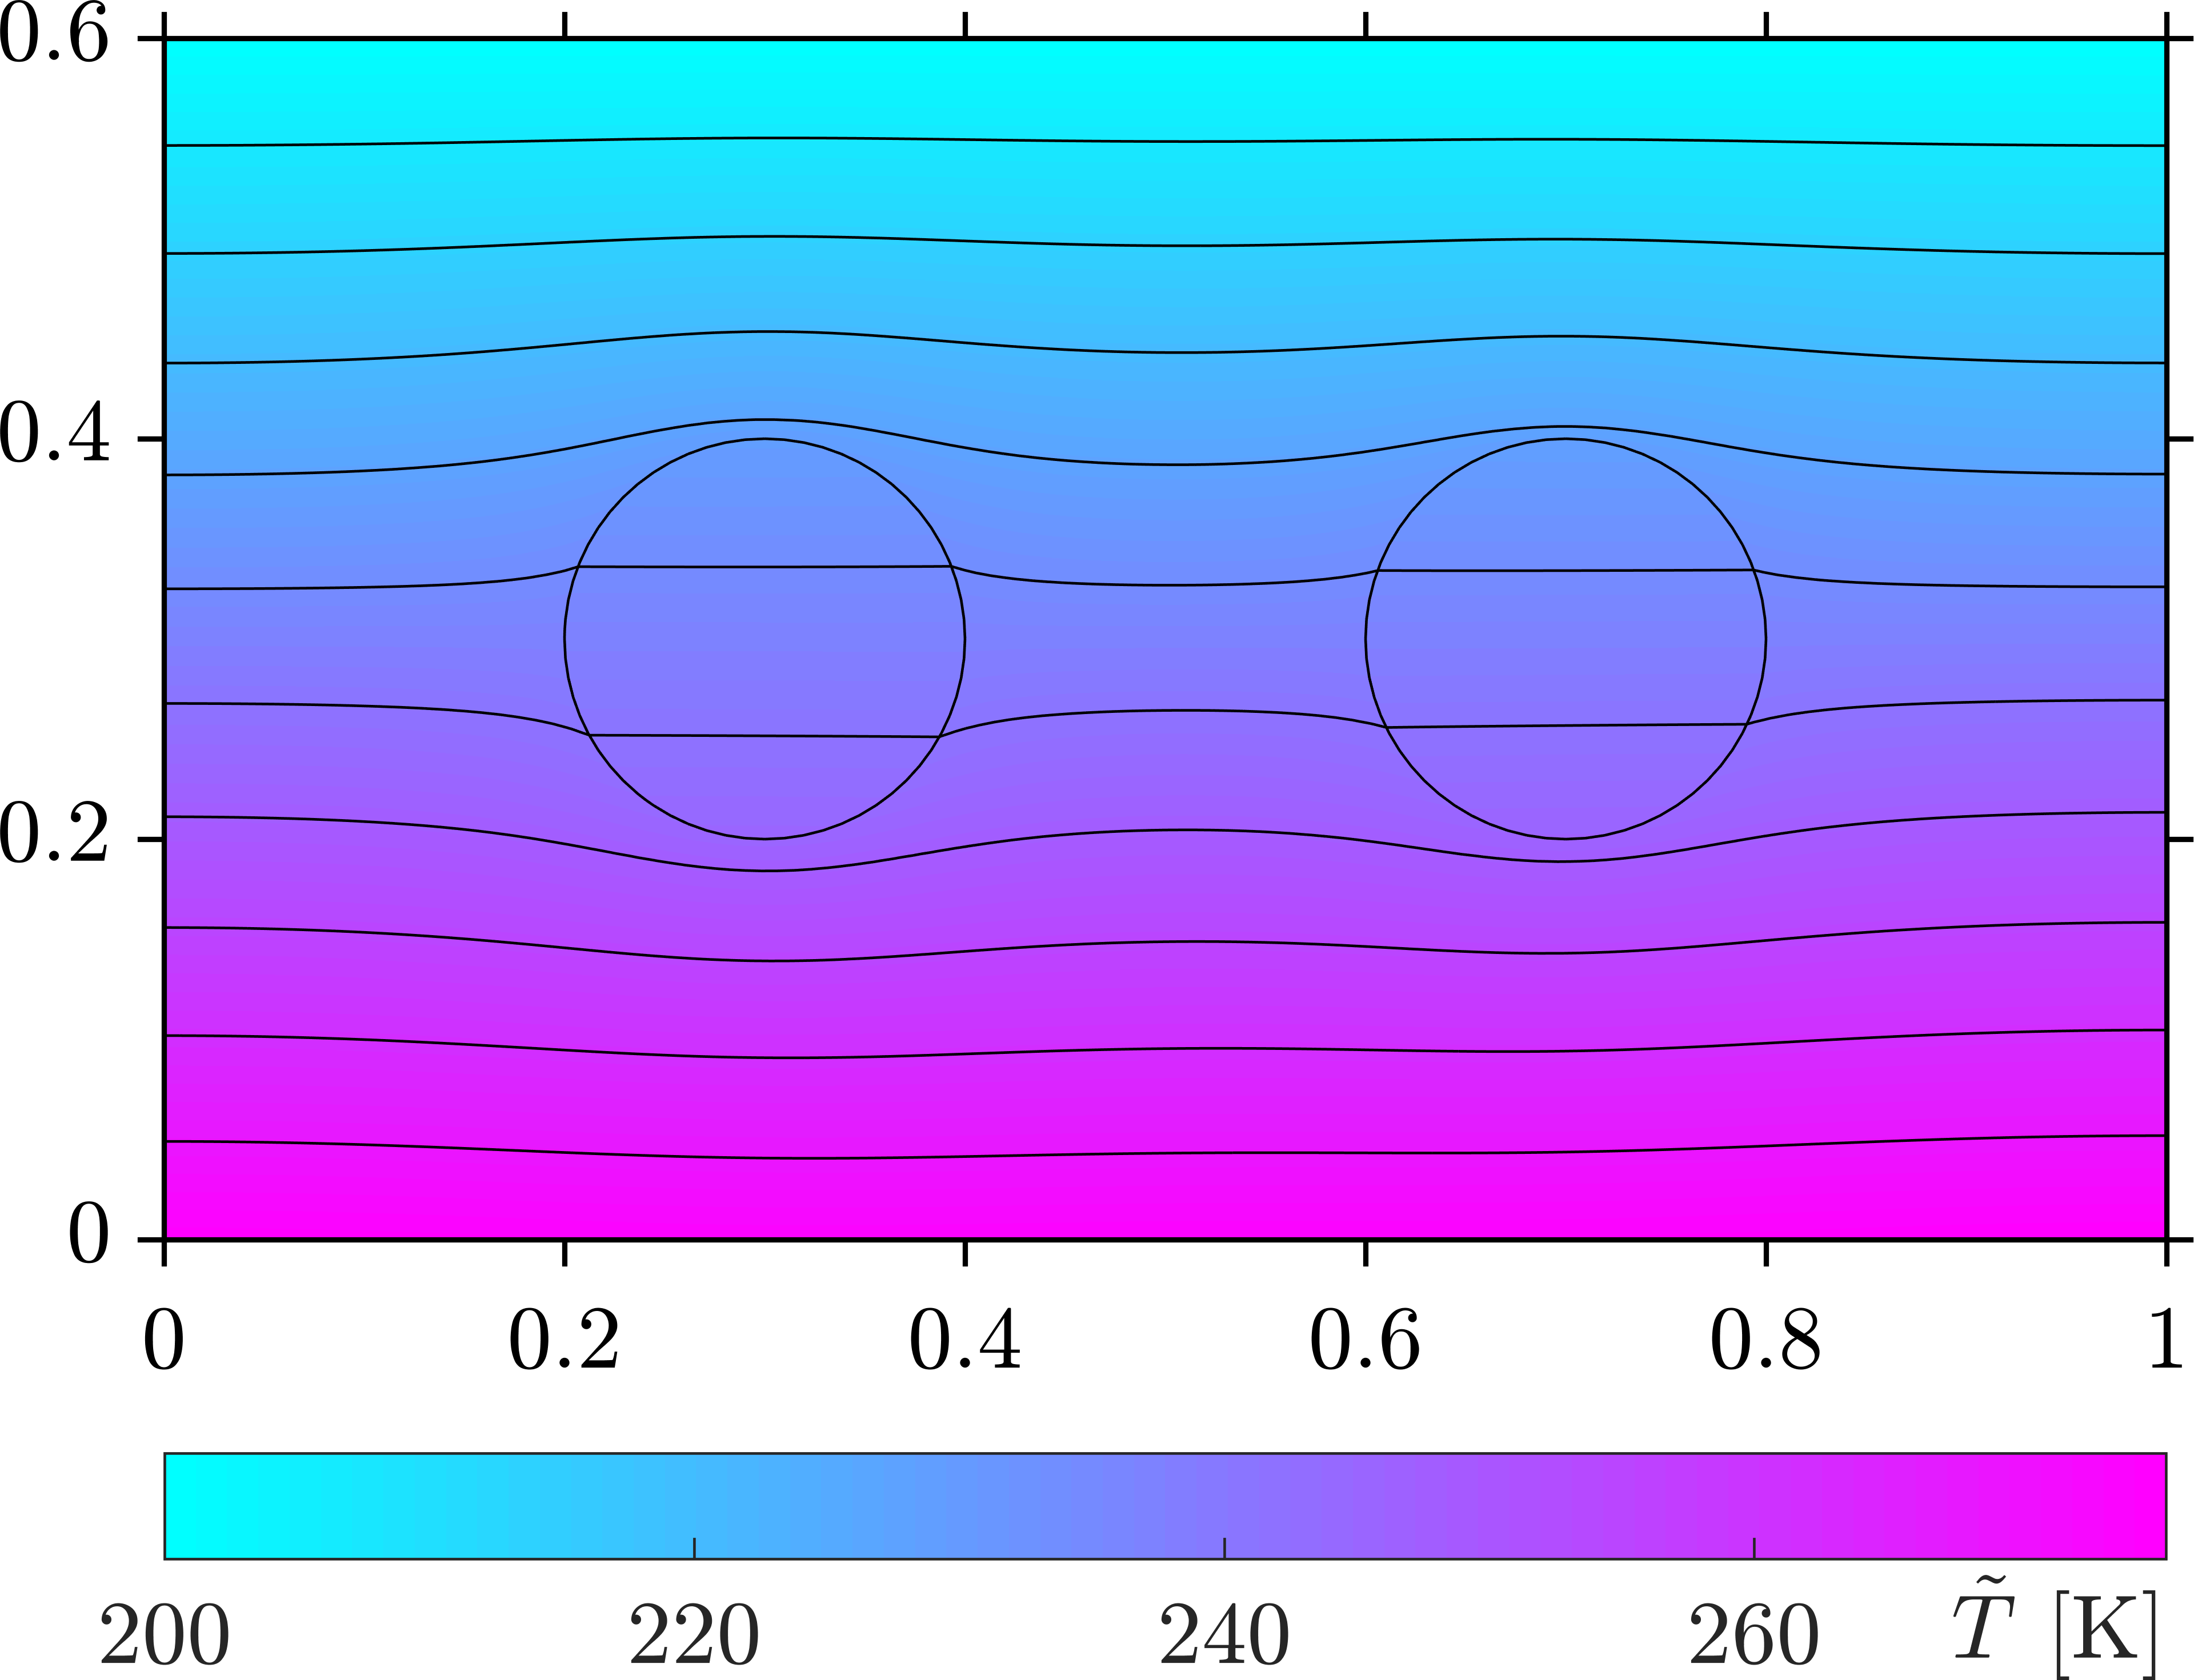
\includegraphics[height=\JCPfigHeight]{fig_JCP_Heat2D_SteadyState}
    \caption[2D IHCP: Steady state solution]{2D IHCP: Steady state solution.}
    \label{fig:JCP:Heat:SteadyState2D}
  \end{minipage}%
\end{figure}

\subsubsection{Posterior density}
% COMPARISON TO 2D GAUSSIAN
The analyses proceed analogously to the preceding section.
By comparing the present IHCP and the non-conjugate Gaussian example, that have a two-dimensional parameter space and uniform priors in common,
one can gain interesting insight into spectral Bayesian inference.
% SLE CONVERGENCE
First, the convergence behavior of the SLE is investigated.
Spectral expansions \(\hat{\mathcal{L}}_p\) of the likelihood \(\mathcal{L}\) are therefore computed
for an experimental design of size \(K = 1 \times 10^5\) and candidate bases with polynomials up to degree \(p = 50\).
All practical issues are handled analogously to the procedure in the non-conjugate Gaussian example.
In \cref{fig:JCP:Heat:ConvSLE} the normalized versions of the empirical error \(\epsilon_{\mathrm{Emp}}\) and the LOO error \(\epsilon_{\mathrm{LOO}}\) are shown as a function of \(p\).
Comparing these results to \cref{fig:JCP:Normal:ConvSLE} reveals that the convergence rate of the SLE \(\hat{\mathcal{L}}_p\) is considerably slower than the corresponding one for the Gaussian example.
For the SLE with \(p = 50\) the error estimates amount to \(\epsilon_{\mathrm{Emp}} = 6.26 \times 10^{-4}\) and \(\epsilon_{\mathrm{LOO}} = 7.56 \times 10^{-4}\).
These errors are around seven orders of magnitude higher than the errors observed for the Gaussian example.
% DIFFERENT CONVERGENCE RATE
The difference in the SLE convergence rate presumably originates from a difference in the underlying likelihood functions and posterior densities.
This is now investigated in more detail.
% FIGURE: SLE CONVERGENCE
\begin{figure}[htbp]
  \centering
  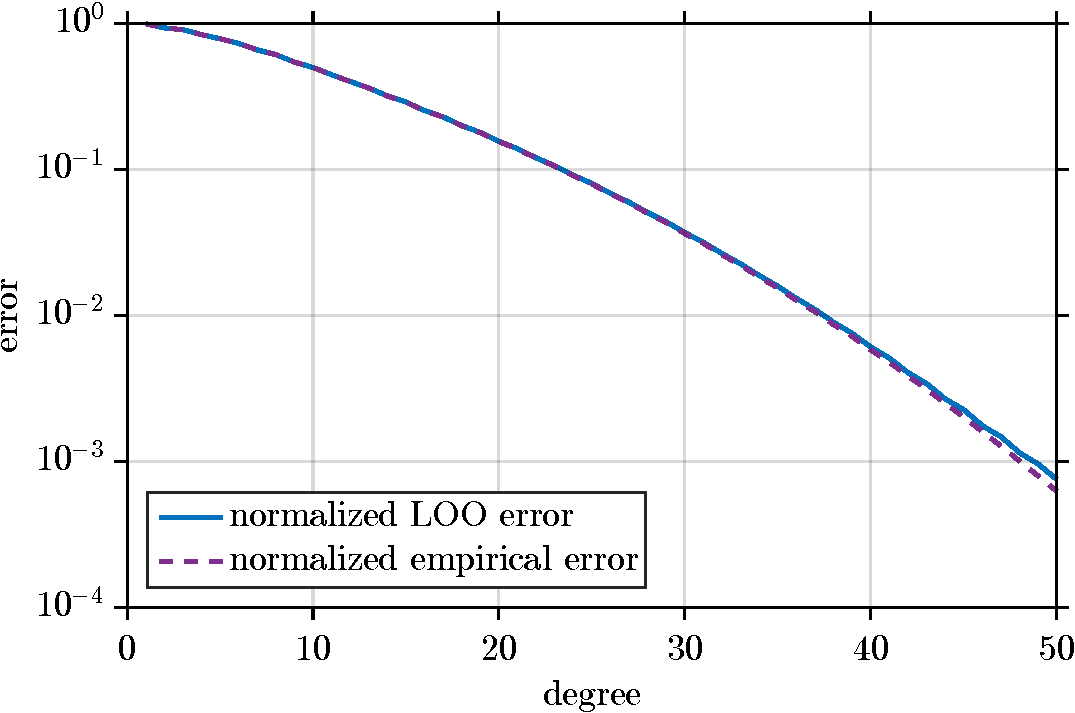
\includegraphics[height=\JCPfigHeight]{fig_JCP_Heat2D_ConvSLE}
  \caption[2D IHCP: Convergence of the SLE]{2D IHCP: Convergence of the SLE.}
  \label{fig:JCP:Heat:ConvSLE}
\end{figure}
\par % POSTERIOR DENSITY
A RWM approximation with \(10^7\) samples and the SLE-based emulation with \(p = 50\) of the posterior density
\(\pi(\kappa_1,\kappa_2 \cond \bm{T}) \approx \coeffL_{\bm{0}}^{-1} \hat{\mathcal{L}}_p(\kappa_1,\kappa_2) \pi(\kappa_1,\kappa_2)\) are depicted in \cref{fig:JCP:Heat:Post2D}.
% FORWARD MODEL SURROGATE
In order to reduce the numerical cost of MCMC sampling, the FE model \(\mathcal{M}\) is replaced by a PCE surrogate \(\hat{\mathcal{M}}_p\).
For \(i = 1,\ldots,\dimData\), separate PCEs \(\hat{\mathcal{M}}_{i,p}\) of the temperature \(\perfect{T}_i = \mathcal{M}_{i,p}(\kappa_1,\kappa_2)\)
at the location \(\bm{r}_i\) are fitted as a function of the unknown conductivities.
After an appropriate transformation to standardized variables, tensorized Legendre polynomials up to degree \(p = 10\) act as the trial basis.
Based on an experimental design of the size \(K = 10^3\), the LOO errors of the regressions amount to about \(\epsilon_{\mathrm{LOO}} \approx 10^{-10}\).
Accordingly, the PCE is considered an adequate replacement of the full FE model.
% TWO-STAGE REGRESSION
Note that it would be also possible to use \(\hat{\mathcal{M}}_p\) as a forward model surrogate during the likelihood training runs.
\par % POSTERIOR DENSITY
The posteriors in \cref{fig:JCP:Heat:Post2D} can be compared to the posteriors of the Gaussian example in \cref{fig:JCP:Normal:Post2D} of the previous section.
Relative to the respective prior, the posterior of the thermal problem \(\pi(\kappa_1,\kappa_2 \cond \bm{T})\)
contains more information than the posterior of the normal problem \(\pi(\mu,\sigma \cond \bm{y})\),
i.e.\ the likelihood \(\mathcal{L}(\kappa_1,\kappa_2)\) has a slightly more peaked and localized structure than \(\mathcal{L}(\mu,\sigma)\).
In order to capture these different behaviors nearby and far from the posterior mode,
the SLEs \(\hat{\mathcal{L}}_p(\kappa_1,\kappa_2)\) and \(\hat{\mathcal{L}}_p(\mu,\sigma)\) require a different number of expansions terms.
The more localized the posterior modes are with respect to the prior, the more terms are required in order to achieve the cancellation in the tails.
Moreover, as opposed to \(\pi(\mu,\sigma \cond \bm{y})\) the posterior \(\pi(\kappa_1,\kappa_2 \cond \bm{T})\) exhibits a pronounced correlation structure.
In turn, this requires non-vanishing interaction terms.
As a consequence, the SLE \(\hat{\mathcal{L}}_p(\kappa_1,\kappa_2)\) of the IHCP example is less accurate than the SLE \(\hat{\mathcal{L}}_p(\mu,\sigma)\) of the Gaussian example.
This is also reflected in the fact that the posterior surrogate fluctuates and takes on negative values
around the points \([\underline{\kappa}_1,\underline{\kappa}_2]\) and \([\overline{\kappa}_1,\overline{\kappa}_2]\).
In order to see this more clearly, the SLE posterior surrogate from \cref{fig:JCP:Heat:Post2D:SLE} is plotted again from a different angle in \cref{fig:JCP:Heat:Post3D:SLE}.
A small wavelike posterior structure spans the parameter space between these corners.
These artifacts stem from an imperfect polynomial cancellation of the finite series approximation.
This stands in contrast to the posterior of the Gaussian example in \cref{fig:JCP:Normal:Post3D:SLE} where these phenomena were not observed.
% FIGURES: 2D POSTERIORS
\begin{figure}[htbp]
  \centering
  \begin{subfigure}[b]{\JCPsubWidth}
    \centering
    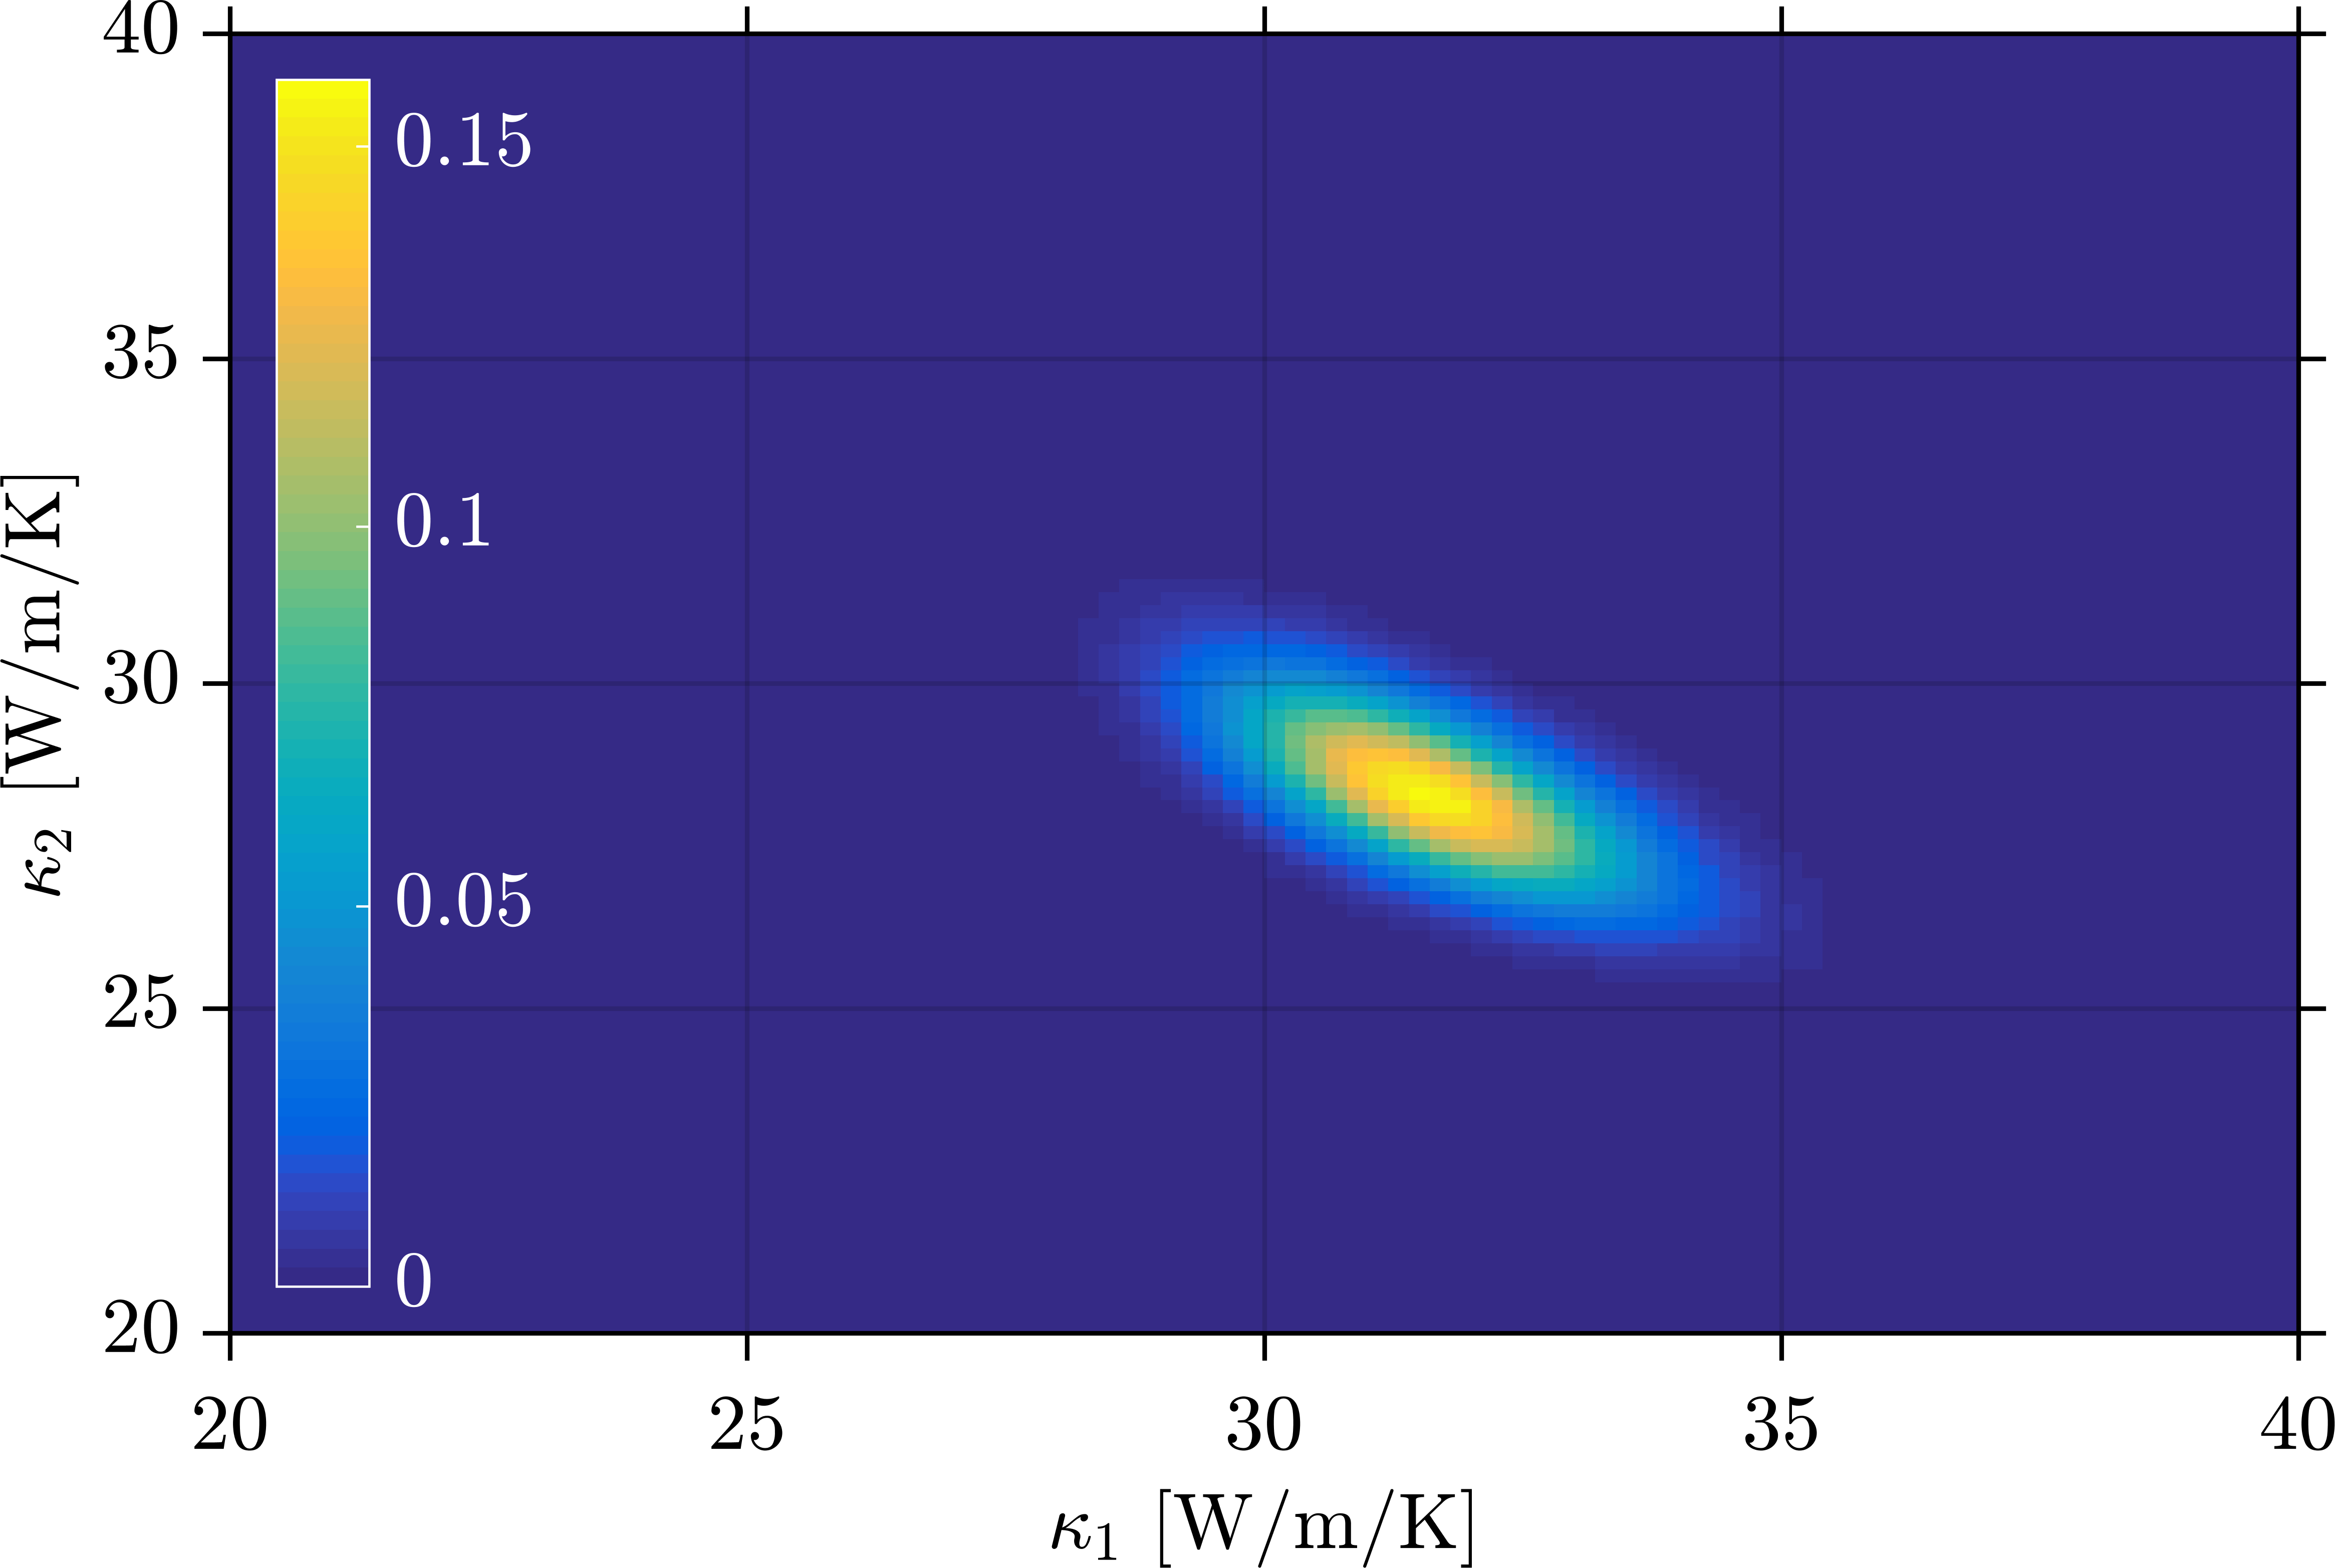
\includegraphics[height=\JCPfigHeight]{fig_JCP_Heat2D_Post2D_MCMC}
    \caption{MCMC reference sample.}
    \label{fig:JCP:Heat:Post2D:MCMC}
  \end{subfigure}\hfill%
  \begin{subfigure}[b]{\JCPsubWidth}
    \centering
    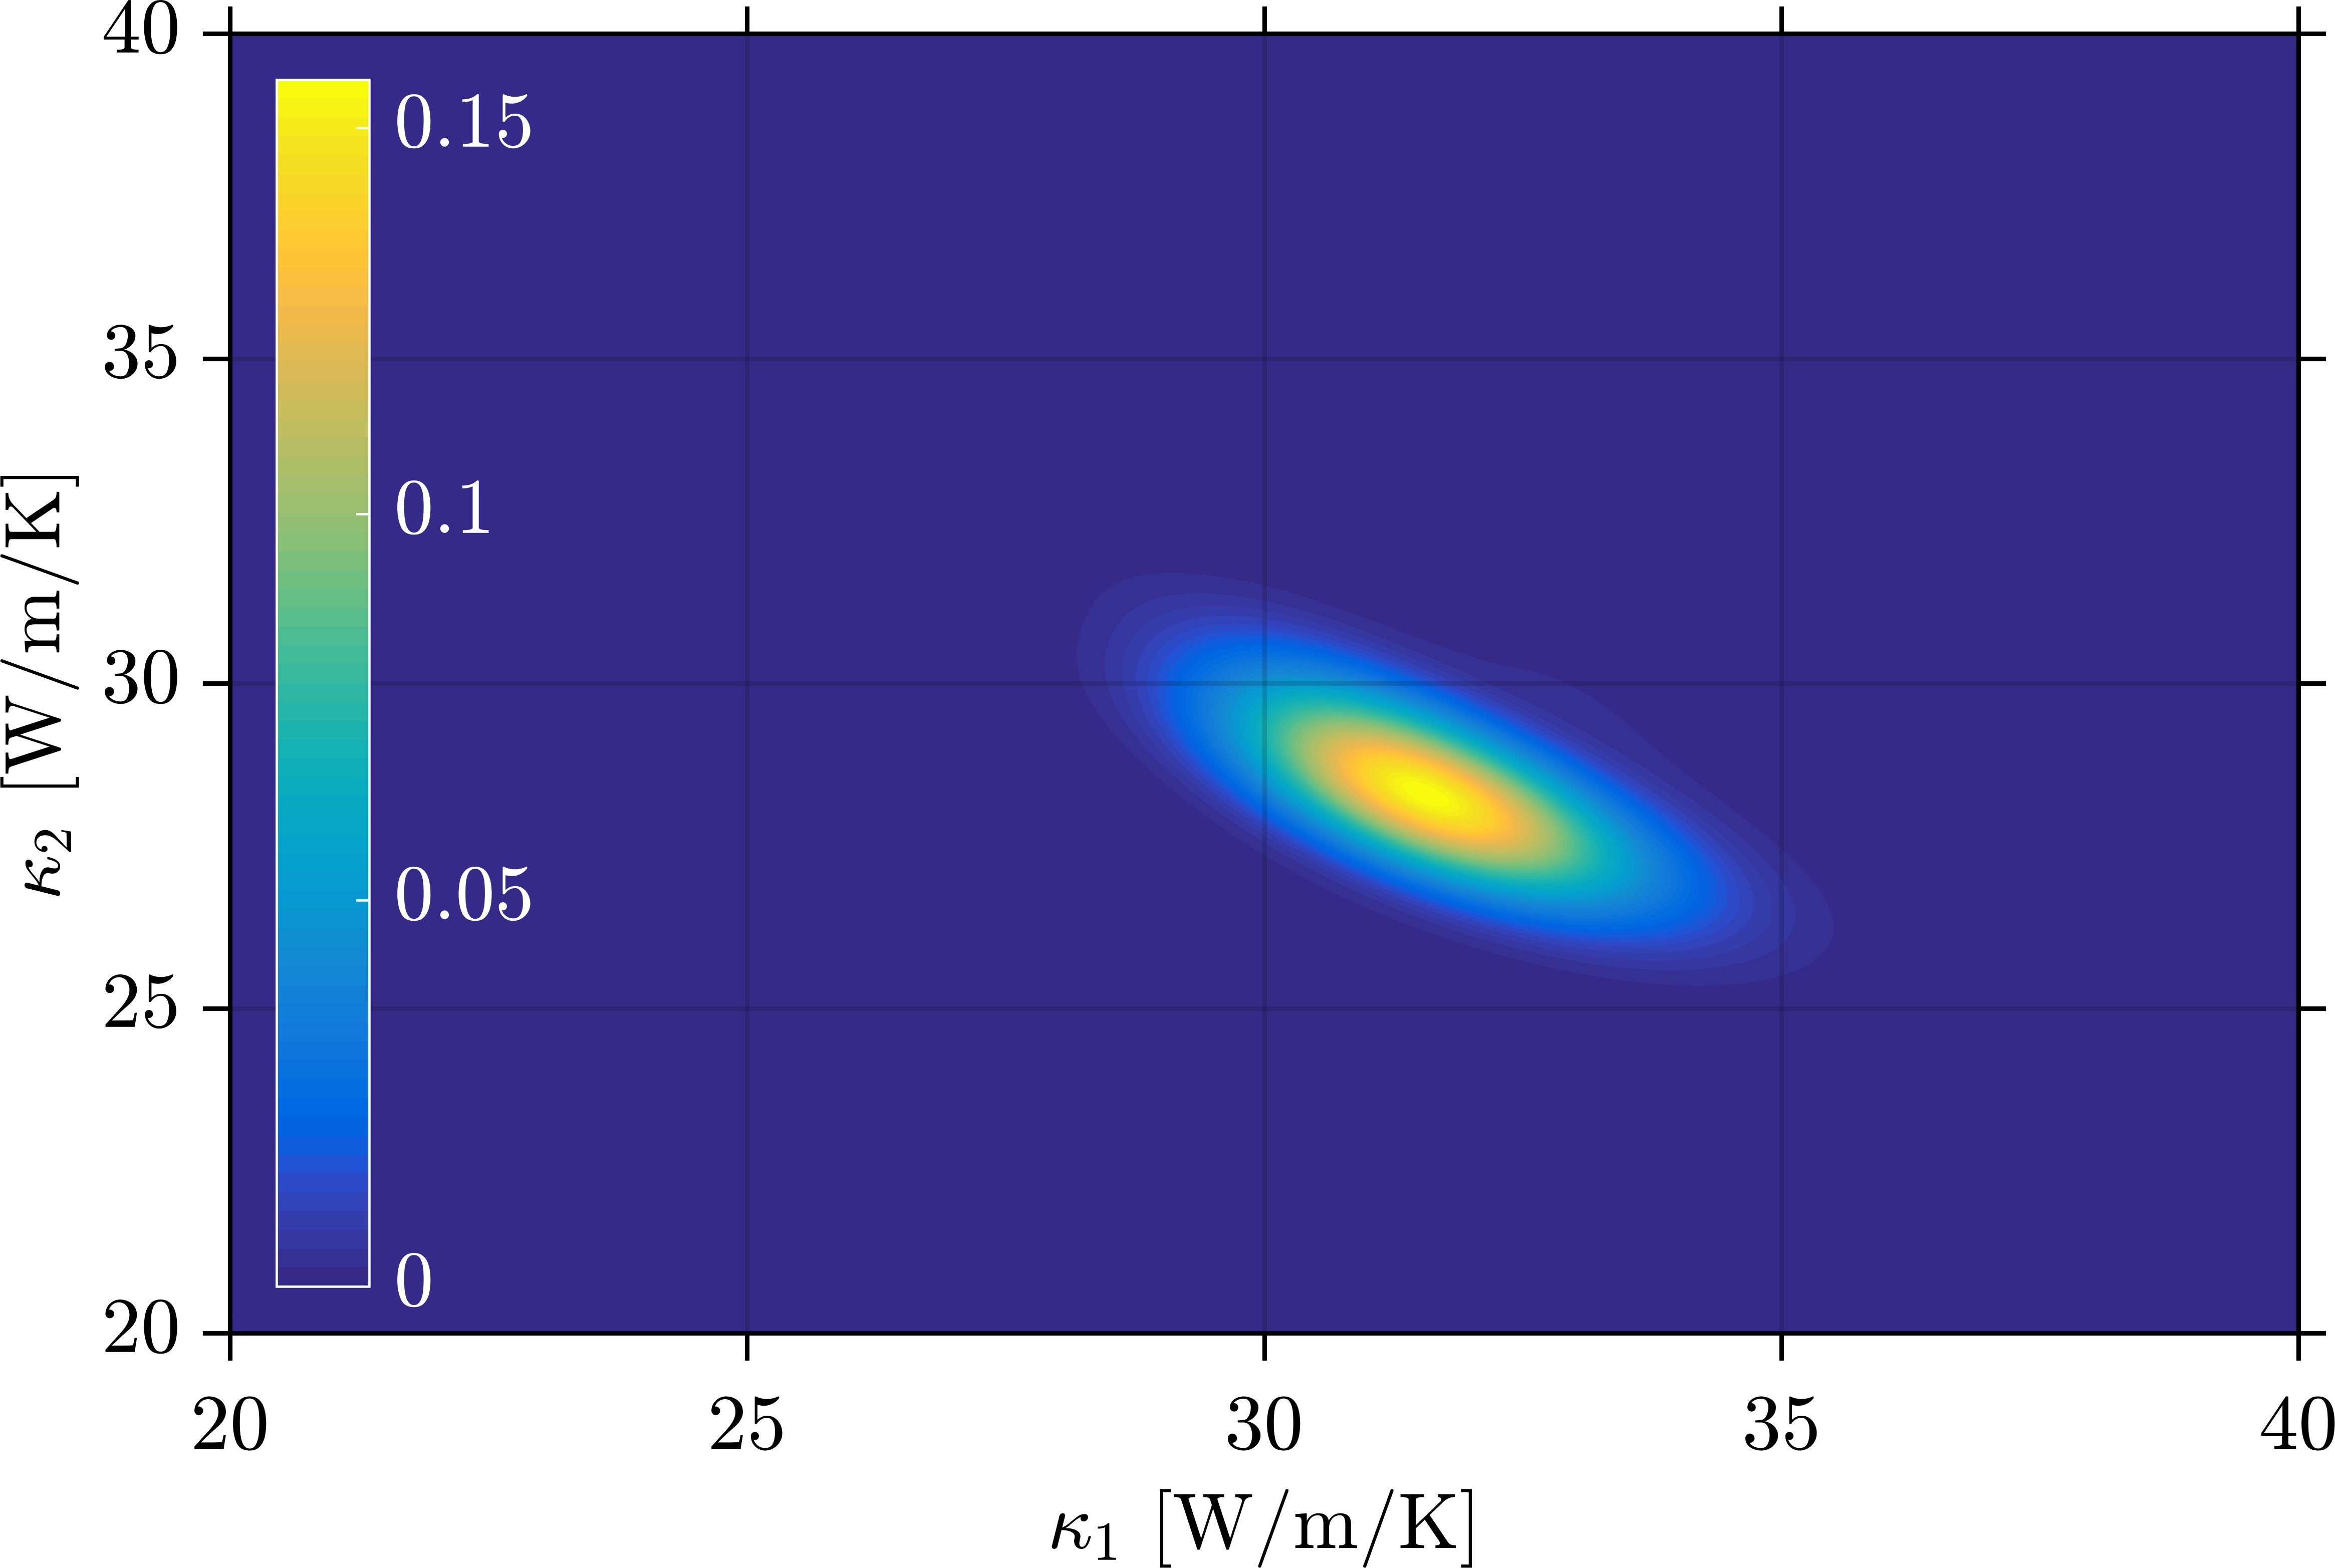
\includegraphics[height=\JCPfigHeight]{fig_JCP_Heat2D_Post2D_SLE}
    \caption{SLE with \(p = 50\).}
    \label{fig:JCP:Heat:Post2D:SLE}
  \end{subfigure}\\[1ex]%
  \begin{subfigure}[b]{\JCPsubWidth}
    \centering
    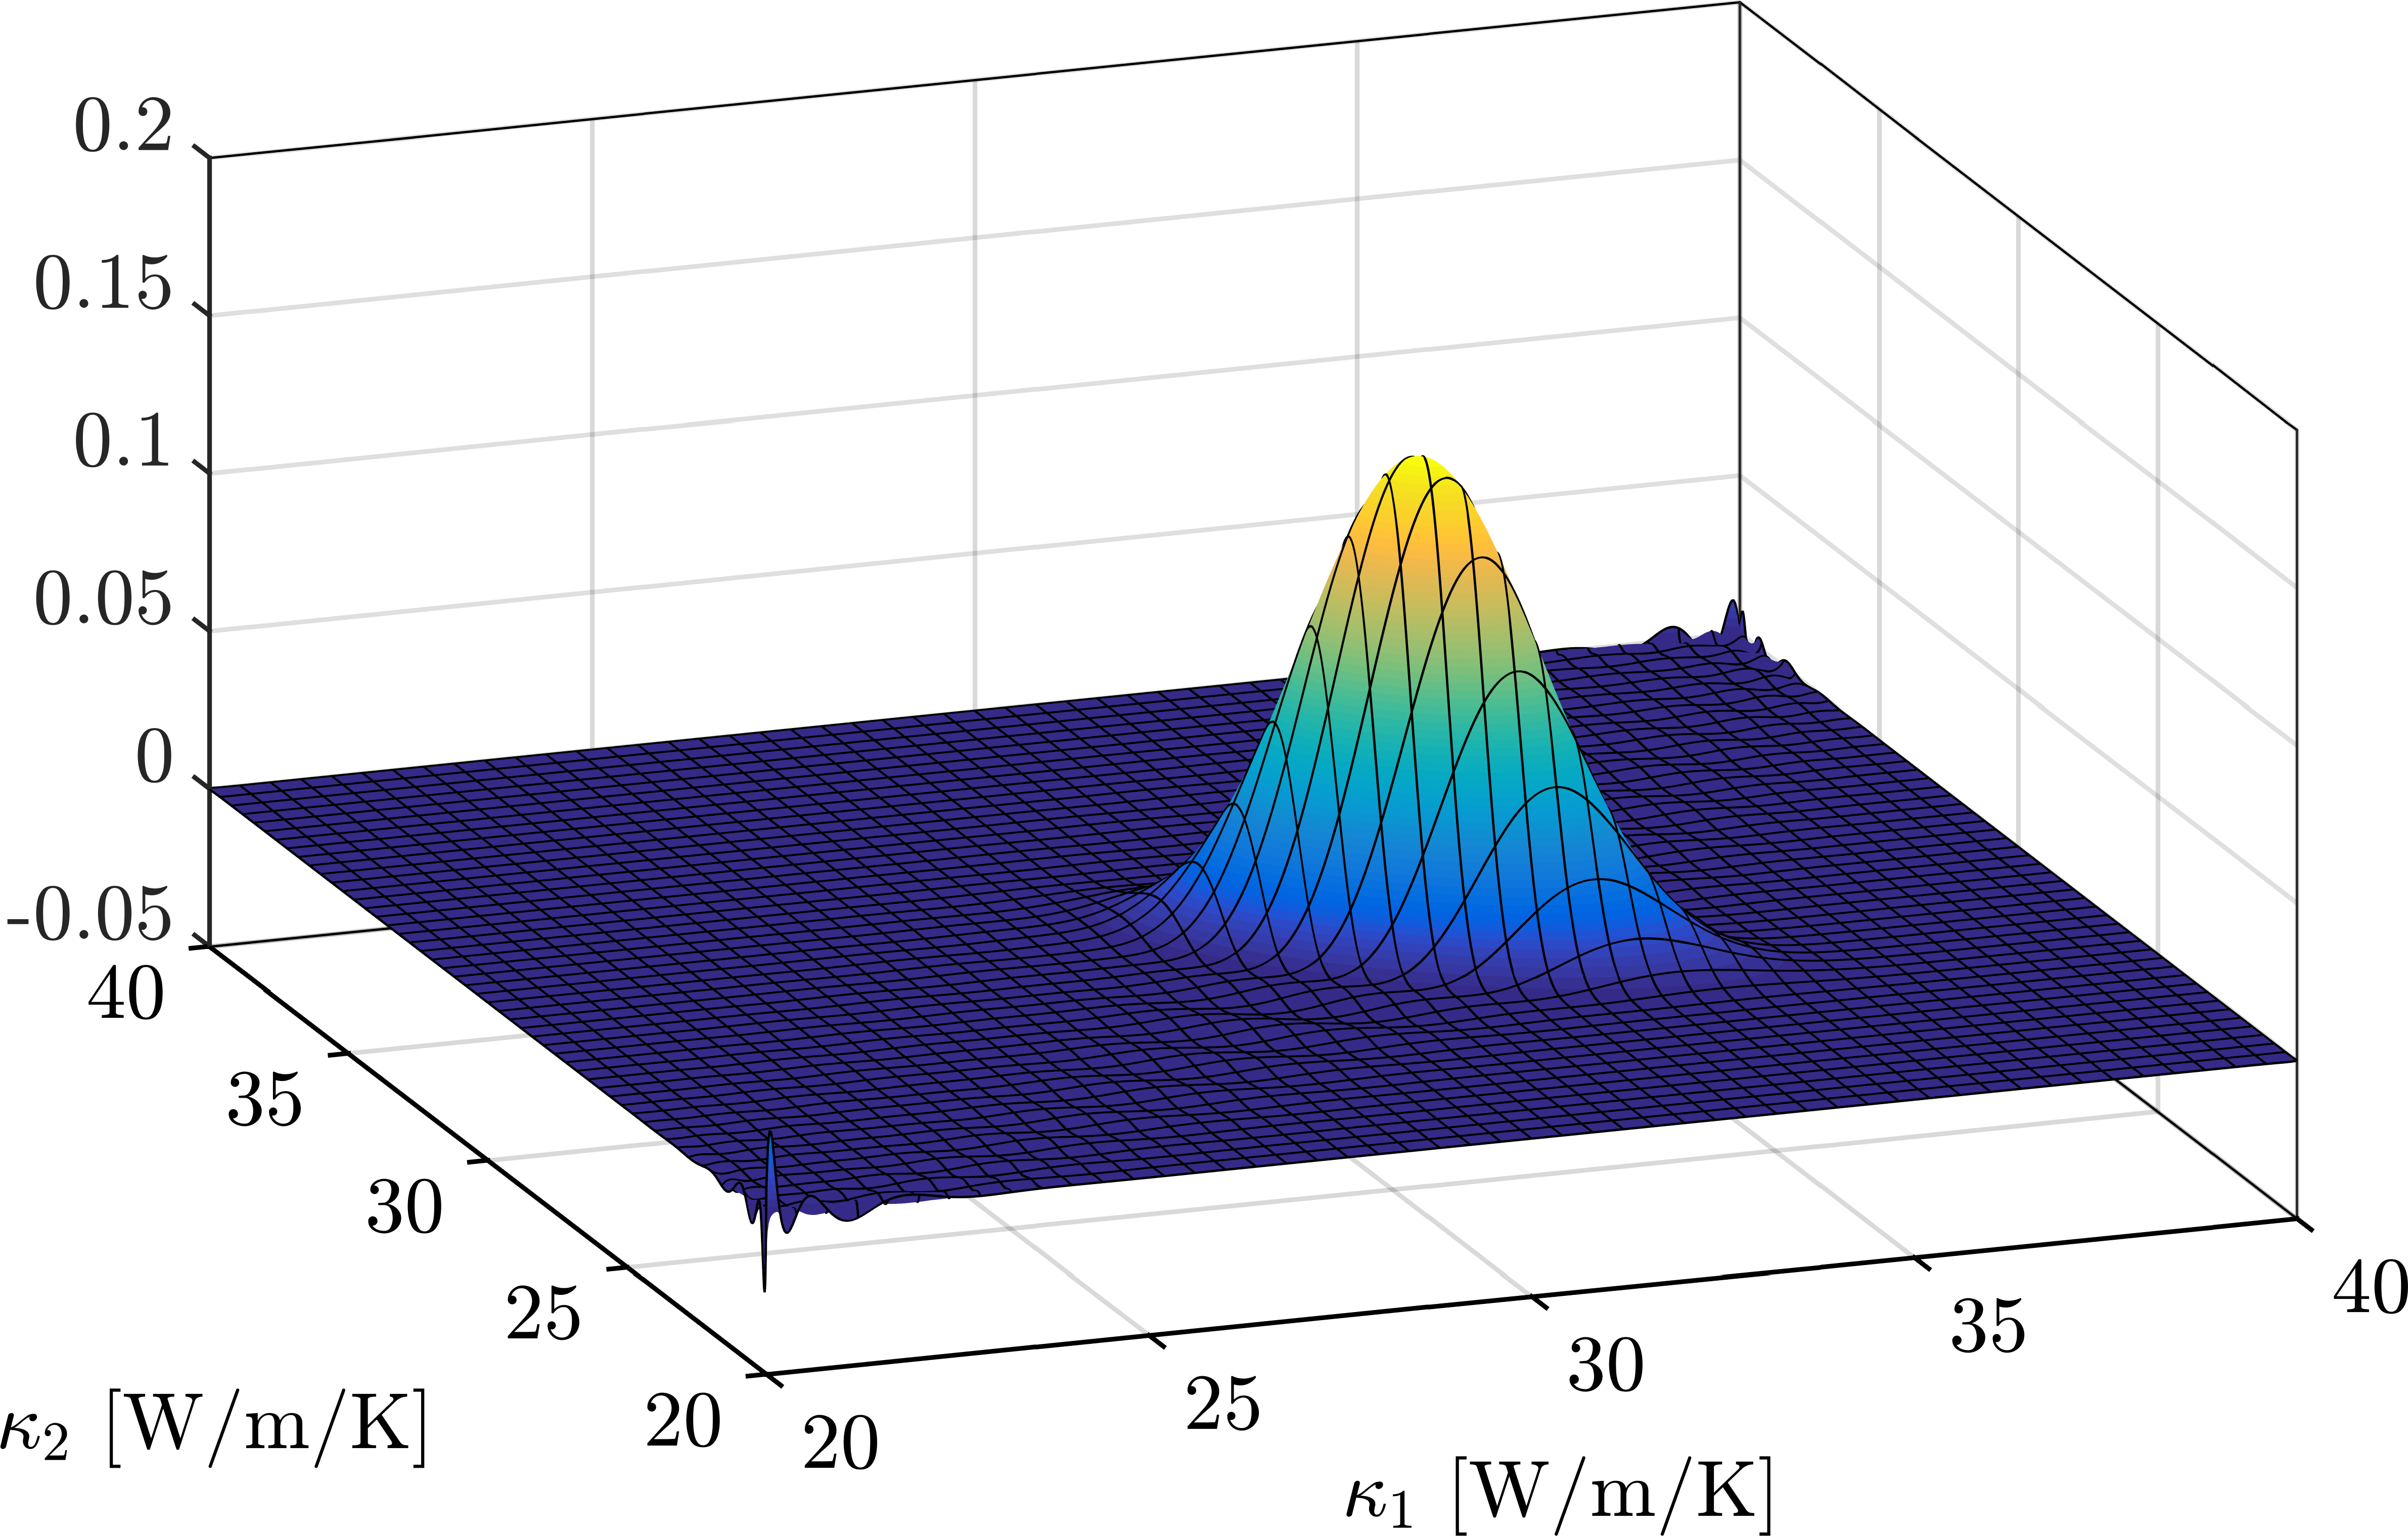
\includegraphics[width=\JCPfigWidth]{fig_JCP_Heat2D_Post3D_SLE}
    \caption{SLE with \(p = 50\).}
    \label{fig:JCP:Heat:Post3D:SLE}
  \end{subfigure}%
  \caption[2D IHCP: Joint posterior]{2D IHCP: Joint posterior.}
  \label{fig:JCP:Heat:Post2D}
\end{figure}
\par % POSTERIOR MARGINALS
Via \cref{eq:JCP:SLE:Marginal1D} the posterior marginals \(\pi(\kappa_1 \cond \bm{T})\) and \(\pi(\kappa_2 \cond \bm{T})\) can be extracted from the joint SLEs.
The resulting densities are shown in \cref{fig:JCP:Heat:Post1D} together with a histogram-based MCMC sample representation.
As it can be seen, for \(p = 50\) the marginals are captured fairly well,
while the moderate-order surrogate for \(p = 21\) still exhibits discrepancies at the bounds of the parameter space.
The approximation of the posterior marginals by sub-SLEs seems to be more accurate, at least in the sense of the maximum deviation,
than the approximation of the joint posterior \(\pi(\kappa_1,\kappa_2 \cond \bm{T})\) by the full SLE in \cref{fig:JCP:Heat:Post3D:SLE}.
This phenomenon can be explained through the absence of all non-constant polynomial terms in the variables that are marginalized out.
% FIGURES: POSTERIOR MARGINALS
\begin{figure}[htbp]
  \centering
  \begin{subfigure}[b]{\JCPsubWidth}
    \centering
    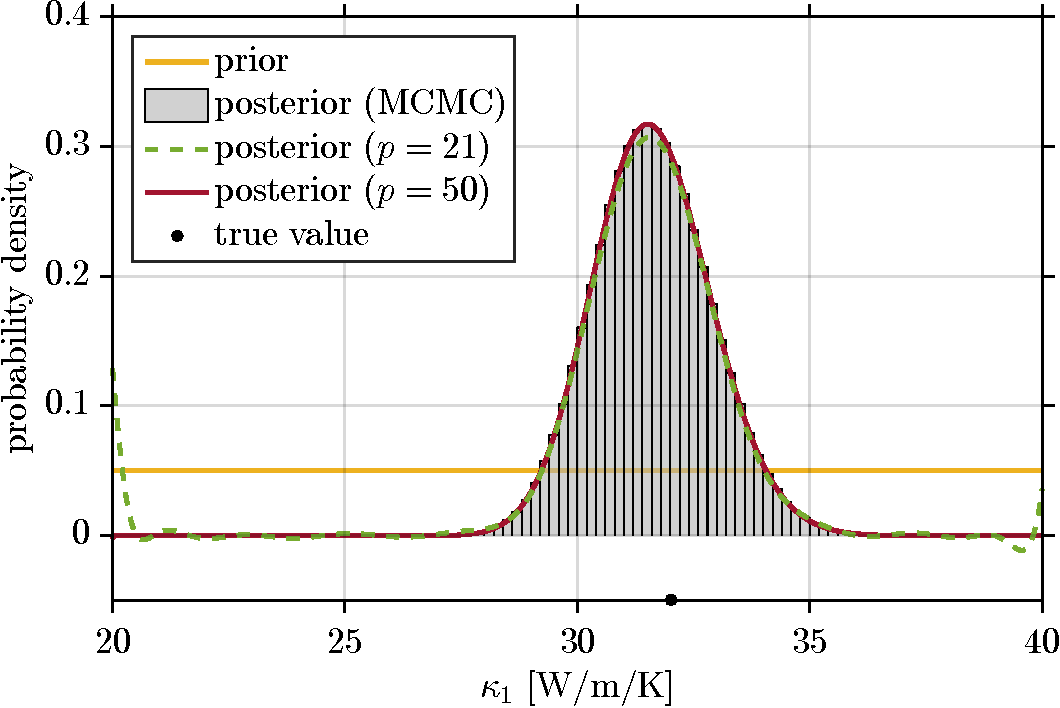
\includegraphics[height=\JCPfigHeight]{fig_JCP_Heat2D_Post1D_k1}
    \caption{Thermal conductivity \(\kappa_1\).}
    \label{fig:JCP:Heat:Post1D:k1}
  \end{subfigure}\hfill%
  \begin{subfigure}[b]{\JCPsubWidth}
    \centering
    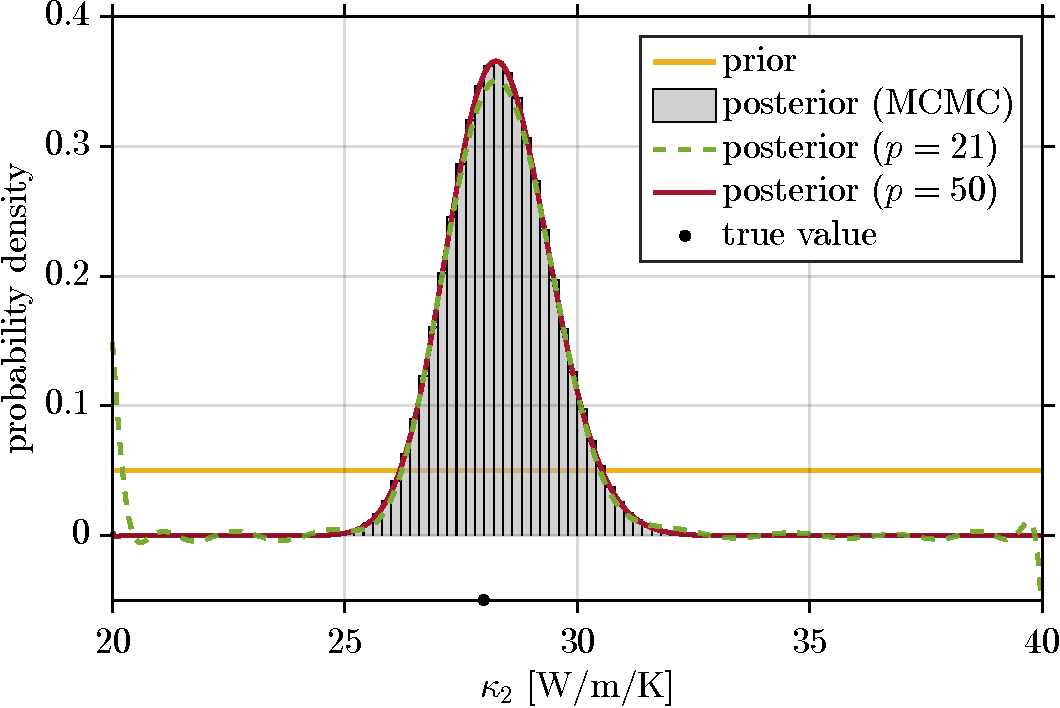
\includegraphics[height=\JCPfigHeight]{fig_JCP_Heat2D_Post1D_k2}
    \caption{Thermal conductivity \(\kappa_2\).}
    \label{fig:JCP:Heat:Post1D:k2}
  \end{subfigure}%
  \caption[2D IHCP: Posterior marginals]{2D IHCP: Posterior marginals.}
  \label{fig:JCP:Heat:Post1D}
\end{figure}

\subsubsection{Quantities of interest}
% STATISTICAL QUANTITIES OF INTEREST
Now we investigate how well one can extract the statistically interesting quantities.
Results from SLEs with varying \(K\) and \(p\) are compared with the results from MCMC sampling.
A summary of the findings is provided in \cref{tab:JCP:Heat:StatisticalQuantities}.
The LOO error \(\epsilon_{\mathrm{LOO}}\) of various SLEs is shown together with some basic posterior characteristics obtained by a postprocessing of the SLE coefficients.
For \(j = 1,2\) the posterior mean \(\mathds{E}[\kappa_j \cond \bm{T}]\) and the standard deviation \(\mathrm{Std}[\kappa_j \cond \bm{T}] = \mathrm{Var}[\kappa_j \cond \bm{T}]^{1/2}\)
of the posterior distribution are given in physical units of \(\unit[]{W/m/K}\).
In addition, the model evidence \(\scale\) and the linear coefficient of correlation
\(\rho[\kappa_1,\kappa_2 \cond \bm{T}] = \mathrm{Cov}[\kappa_1,\kappa_2 \cond \bm{T}] / \mathrm{Std}[\kappa_1 \cond \bm{T}] / \mathrm{Std}[\kappa_2 \cond \bm{T}]\) are specified.
% DISCUSSION
In comparison to \cref{tab:JCP:Normal:StatisticalQuantities}, where the results for the non-conjugate normal example are listed, the SLE results for the IHCP match their MCMC counterparts less accurately.
Nevertheless, it can be observed that the lowest-degree quantities of inferential interest can be extracted with a comparably small experimental design and relatively low number of regressors,
say with \(K = 1 \times 10^4\) and \(p = 29\).
Note that all the estimates attain admissible values.
% TABLE: STATISTICAL QUANTITIES
\begin{table}[htbp]
  \caption[2D IHCP: Statistical quantities]{2D IHCP: Statistical quantities.}
  \label{tab:JCP:Heat:StatisticalQuantities}
  \centering
  \begin{tabular}{cccccccccc}
    \toprule
    & \(K\) & \(p\) & \(\epsilon_{\mathrm{LOO}}\)
    & \(\scale\) \([10^{-1}]\) & \(\mathds{E}[\kappa_1 \cond \bm{T}]\) & \(\mathds{E}[\kappa_2 \cond \bm{T}]\)
    & \(\mathrm{Std}[\kappa_1 \cond \bm{T}]\) & \(\mathrm{Std}[\kappa_2 \cond \bm{T}]\) & \(\rho[\kappa_1,\kappa_2 \cond \bm{T}]\) \\
    \midrule
    \multirow{6}{*}{\rotatebox[origin=c]{90}{SLE}}
    & \(5 \times 10^2\) & \(5\)  & \(8.24 \times 10^{-1}\) & \(8.45\) & \(31.33\) & \(28.36\) & \(1.74\) & \(1.33\) & \(\phantom{-}0.28\) \\
    & \(1 \times 10^3\) & \(9\)  & \(6.08 \times 10^{-1}\) & \(7.81\) & \(31.40\) & \(28.22\) & \(2.02\) & \(1.53\) & \(\phantom{-}0.15\) \\
    & \(5 \times 10^3\) & \(21\) & \(1.50 \times 10^{-1}\) & \(7.47\) & \(31.32\) & \(28.13\) & \(2.16\) & \(1.61\) & \(\phantom{-}0.34\) \\
    & \(1 \times 10^4\) & \(29\) & \(5.79 \times 10^{-2}\) & \(7.21\) & \(31.56\) & \(28.30\) & \(1.61\) & \(1.39\) & \(-0.05\) \\
    & \(5 \times 10^4\) & \(35\) & \(1.63 \times 10^{-2}\) & \(7.18\) & \(31.62\) & \(28.34\) & \(1.24\) & \(1.08\) & \(-0.75\) \\
    & \(1 \times 10^5\) & \(50\) & \(7.56 \times 10^{-4}\) & \(7.18\) & \(31.62\) & \(28.33\) & \(1.26\) & \(1.10\) & \(-0.68\) \\
    \midrule
    \multicolumn{4}{c}{(MC)MC}                             & \(7.17\) & \(31.62\) & \(28.33\) & \(1.26\) & \(1.09\) & \(-0.68\) \\
    \bottomrule
  \end{tabular}
\end{table}